\chapter{Introduction}
The goal of this lab is to implement performance-enhancing circuitry that is difficult to express in C, but can be done in very parallel fashion in hardware (\verb|vhdl| design) for example bit operations like reshuffling within several bytes. Showed techniques can be utilised for the program parts which take a lot of time and processor resources to execute. These parts can be discovered in the profiling process and finally implemented in hardware either as the custom instructions or hardware accelerators. For the sake of this project the bit reshuffling will be implemented using those three approaches, (full software, custom instruction and hardware accelerator) and compared using profiling tools to judge which solution is the best from the execution time point of view. As an attachment to this report, authors provided packed sources, that is hardware design, \verb|qsys| file, and software. \footnote{Unfortunately software is kept in the hardware directory, because authors faced some problems with bsp generation if, software was placed in the different destination then the default one}. 

\begingroup
\renewcommand{\cleardoublepage}{}
\renewcommand{\clearpage}{}
\chapter{Software bit swapping}
\endgroup
In this part the bit swapping has been done by software. The calculation to perform is the following. Every bit within 4 middle bytes will be reshuffled, that is for example 0111 0011 1010 1100 will become 0011 0101 1100 1110. 2 most significant bytes, will be replaced with 2 least one, and vice versa. For example 0x12345678 will become 0x786a2c12.
\section{System configuration}
The system has two caches enabled. In the first one instruction cache has 4kB and data cache 2kB. In addition the system uses internal onchip memory. \figurename{} \ref{fig:system1} shows the connections between every component for that part of the project. 
\begin{figure}[H]
	\begin{center}
		\scalebox{0.5}{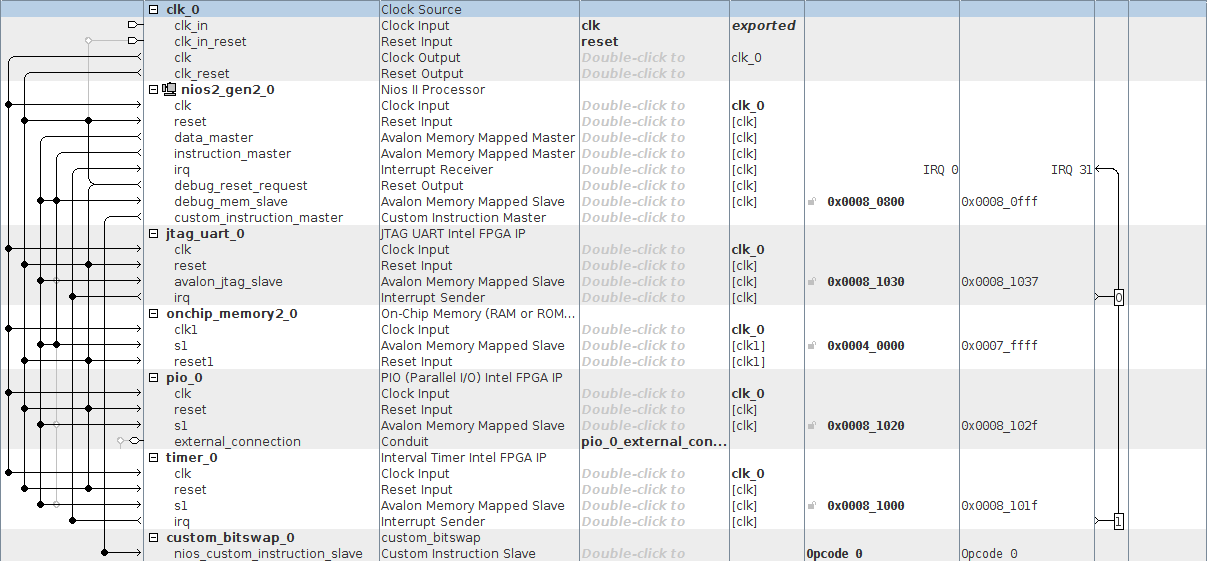
\includegraphics{./pictures/QSYS_CI.png}}
	\end{center}
	\caption{System connections for the software part and the custom instruction}

	\label{fig:system1}
\end{figure}

Following listing shows two functions responsible for the bit swapping logic. Quick conclusion is that the bit operations are not trivial. Every bit has to be swapped separately (\verb|SwapTP2|, but this part can be implemented also in the loop), in addition the bit operation itself are not simple -- \verb|Swap| function. 
\begin{lstlisting}[style=customc, frame=none]
int SwapTP2(uint32_t res)
{
    res = Swap(24, 0, res);
    res = Swap(25, 1, res);
    res = Swap(26, 2, res);
    res = Swap(27, 3, res);
    res = Swap(28, 4, res);
    res = Swap(29, 5, res);
    res = Swap(30, 6, res);
    res = Swap(31, 7, res);
    
    res = Swap(23, 8, res);
    res = Swap(22, 9, res);
    res = Swap(21, 10, res);
    res = Swap(20, 11, res);
    res = Swap(19, 12, res);
    res = Swap(18, 13, res);
    res = Swap(17, 14, res);
    res = Swap(16, 15, res);
}

int Swap(int a, int b, int data)
{
    if (((data & (1 << a)) >> a) ^ ((data & (1 << b)) >> b))
    {
        n ^= (1 << q        n ^= (1 << p);
    }

    return n;
}
\end{lstlisting}
And a main function, which invokes in the for loop \verb|SwapTP2| function with a random value as an argument.
\begin{lstlisting}[style=customc, frame=none]
int main() {
    uint32_t res;
    int i = 0;
    int lim = 10000;
    for (i = 0; i < lim; i++)
    {
        res = rand();
        res = SwapTP2();
    }
}
\end{lstlisting}

Table \ref{table:softwareCodeMeasure} contains all the measurements gathered by a software profiler. It is worth noting, that the profiler requires a timer defined in the \verb|qsys| file, which connection can be seen on \figurename{} \ref{fig:system1}.

\begin{table}[h!]
\centering
\begin{tabular}{    |l|c|c|c|c|c|c|c|  }
\hline
 Amount of bit swaps & 1 & 10 & 100 & 1'000 & 10'000 & 100'000 & 1'000'000\\
 \hline
 Time spent in function [ms]  & $<$ 1  & $<$ 1  & $<$ 1 & 20 & 200 & 2'050 & 20'530\\
 \hline
\end{tabular}
 \caption{Measurements of different quantity of 32-bits values bit swapped performed in software}
\label{table:softwareCodeMeasure}
\end{table}
The speed of bit swapping is very slow compared to the custom instruction and the accelerator module. This is going to be discussed in the next chapters.

\begingroup
\renewcommand{\cleardoublepage}{}
\renewcommand{\clearpage}{}
\chapter{Custom instruction}
\endgroup

The custom instruction has been built in the \verb|qsys| system using a custom IP component that has two data wires : \verb|dataa| and \verb|result| that are used in the \verb|nios_custom_instruction_bus|. Where dataa is the input data and result the output data that has the bits swapped.

\begin{figure}[H]
	\begin{center}
		\scalebox{0.8}{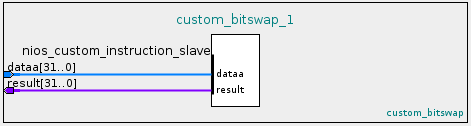
\includegraphics{./pictures/IP_CI.png}}
	\end{center}
	\caption{Custom instruction IP component block diagram}
	\label{fig:customInstruction_blockDiagram}
\end{figure}

 Below is the entity definition for the bit swap that has the connection seen in the IP component on the \figurename{} \ref{fig:customInstruction_blockDiagram}.

\begin{minted}{vhdl}
ENTITY BitSwap IS
PORT(
    dataa	: IN   std_logic_vector( 31 DOWNTO 0);
    result	: OUT  std_logic_vector( 31 DOWNTO 0)    
);
End BitSwap;
\end{minted}

And the architecture of the swapping entity is the following.

\begin{minted}{vhdl}
ARCHITECTURE comp OF BitSwap IS

BEGIN

    result(31 DOWNTO 24) <= dataa(7 DOWNTO 0);
    result(7  DOWNTO 0 ) <= dataa(31 DOWNTO 24);
    PERM: for i in 0 to 15 generate
        result(8+i) <= dataa(23-i);  
    end generate PERM;
	
END comp;
\end{minted}
For the sake of the custom instruction invocation, the specific macro has been defined.
\begin{lstlisting}[style=customc, frame=none]
#define ALT_CI_BITSWAP_N 0x00
#define ALT_CI_BITSWAP(A) __builtin_custom_ini(ALT_CI_BITSWAP_N, (A))
\end{lstlisting}

In the same way as in the full software code, the custom instruction is called in the SwapTP2 function. 
The results of the different times needed for the custom instruction to do the same bit swapping than in the software only version are shown in the table below.

\begin{table}[h!]
\centering
\begin{tabular}{    |l|c|c|c|c|c|c|c|c|c|  }
\hline
 Amount of bit swaps & 1 & 10 & 100 & 1'000 & 10'000 & 100'000 & 1'000'000 & 10'000'000 & 100'000'000 \\
 \hline
 Time in function [ms]  & $<$ 1  & $<$ 1  & $<$ 1 & $<$ 1 & $<$ 1 & 20 & 300 & 2'970 & 29'700\\
 \hline
\end{tabular}
 \caption{Measurements of different quantity of 32-bits values bit swapped in custom instruction}
\label{table:customInstructionCodeMeasure}
\end{table}

The custom instruction is more than 60 times faster than the software code performing exactly the same operation. This timing gain can be very relevant in real time embedded systems, where many computations are performed in the real time and the response should be guaranteed within the specific timing constraint.

\begingroup
\renewcommand{\cleardoublepage}{}
\renewcommand{\clearpage}{}
\chapter{Hardware accelerator}
\endgroup
Hardware accelerator in this case is a \verb|vhdl| design performing the same logic as the C code that is a bit reshuffling, but where several loops and conditions are replaced with finite state machine in hardware description language. In addition the accelerator exchanges data with SDRAM without processor's help, so it is pure \verb|Direct| \verb|Memory| \verb|Access| (\verb|DMA|).

\section{System configuration}

\figurename{} \ref{fig:system} and \ref{fig:addresses} show respectively all the components defined in the system with the connection between them and address map for nios2 processor and hardware accelerator. It is worth noting, that the caches were enabled with following sizes: instruction cache 4kB and data cache 2kB. Also this time as opposite to custom instruction, SDRAM was used instead of onchip memory. 

\begin{sidewaysfigure}

\begin{figure}[H]
	\begin{center}
		\scalebox{0.45}{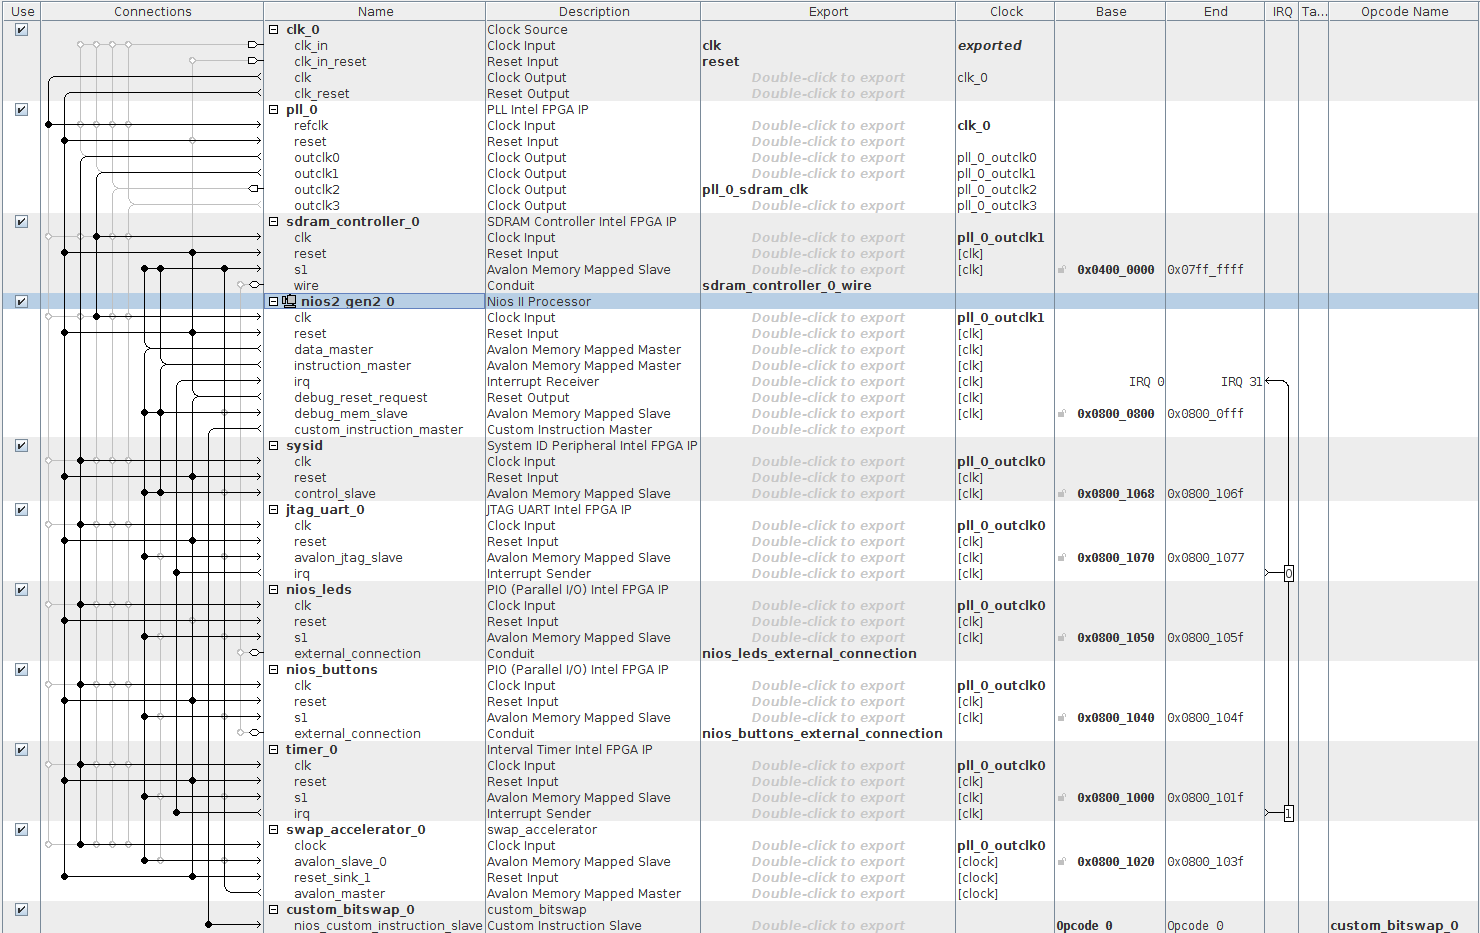
\includegraphics{./pictures/system.png}}
	\end{center}
	\caption{System connections}
	\label{fig:system}
\end{figure}

\end{sidewaysfigure}

\begin{figure}[H]
	\begin{center}
		\scalebox{0.55}{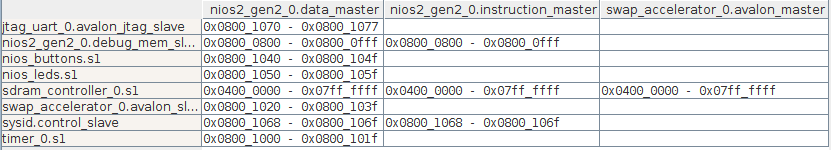
\includegraphics{./pictures/address.png}}
	\end{center}
	\caption{Address map}
	\label{fig:addresses}
\end{figure}


\section{Implementation}
The accelerator defines following entity
\begin{minted}{vhdl}
entity swap is
    port
    (	
    	-- avalon bus
    	Clk             : in  std_logic;
    	nReset          : in  std_logic;
    	-- slave avalon 
    	sAddress        : in  std_logic_vector(2 downto 0);
    	sChipSelect     : in  std_logic;
    	
    	sWrite          : in  std_logic;
    	sWriteData      : in	 std_logic_vector(31 downto 0);
    	sRead           : in  std_logic;
    	sReadData       : out std_logic_vector(31 downto 0);
    	-- master avalon 
    	mAddress        : out  std_logic_vector(31 downto 0);
    	mByteEnable     : out  std_logic_vector(3 downto 0);
    	
    	mWrite          : out  std_logic;
    	mWriteData      : out	 std_logic_vector(31 downto 0);
    	mRead           : out  std_logic;
    	mReadData       : in std_logic_vector(31 downto 0);
    	mWaitRequest    : in  std_logic
    );
end swap;
\end{minted}
Slave signals are signals communicating with the component. They are used in the read and write processes within the architecture to pass data. More specifically these signals are internally used during macro (direct read or write) invocation in the software part. Master signals are used to talk with the \verb|SDRAM| controller.

Next main section in the \verb|vhdl| design is the component's architecture. The internal registers and signals are showed on the following listing
\begin{minted}{vhdl}

signal RegAddStart, RegLgt, Result, 
        ResultRegAddStart           : std_logic_vector(31 downto 0);
signal DataRd                       : std_logic_vector(31 downto 0);
signal start, finish                : std_logic;
signal CntAdd, CntLgt, CntResultAdd : unsigned(31 downto 0);
	
type states_t is (IDLE, LOAD_PARAMETERS, RD_ACC, WAIT_RD, CALCULATE, 
                  SEND_WRITE_REQUEST, WAIT_FOR_WRITE);
signal state : states_t;
\end{minted}
\verb|RegAddStart| and \verb|ResultRegAddStart| are addresses of the source data and result of the computation. \verb|RegLgt| is the length of these data, for example if the size of the array is 10 then the length is simply 10. \verb|Result| keeps the computation result which will be available under \verb|ResultRegAddStart| address. \verb|DataRD| are the data read using master avalon bus directly from the SDRAM, which address is pointed out by \verb|RegAddStart|. \verb|Start| and \verb|Finish| are the status flags. If \verb|Start| is set, then it will be cleared in the next cycle, thereby yielding one-level signal (impulse) only for a brief moment. \verb|Cnt| registers keep the copy of the address registers and their length, they are also unsigned type in order to enable computations like addition or subtraction. Slave writing process is the following
\begin{minted}{vhdl}
slaveWriteProcess : Process(Clk, nReset) 
begin
    if nReset='0' then
        RegAddStart         <= (others => '0');
        RegLgt              <= (others => '0');
        start               <= '0';
        ResultRegAddStart   <= (others => '0');
    
    elsif rising_edge(Clk) then
        start <= '0'; -- in FSM, there is no zeroing Start,
                      -- by doing that here Start is an impuls
        if sChipSelect = '1' and sWrite = '1' then
            case sAddress is
                when "000" => RegAddStart       <= sWriteData; 
                when "001" => RegLgt            <= sWriteData; 
                when "010" => start             <= sWriteData(0); 
                when "011" => ResultRegAddStart <= sWriteData;
                when others => null;
            end case;
        end if;
    end if;
end process slaveWriteProcess;
\end{minted}
And the read process
\begin{minted}{vhdl}
slaveReadProcess : process(Clk) 
begin
    if rising_edge(Clk) then
        if sChipSelect = '1' and sRead = '1' then
            sReadData <= (others => '0');
            case sAddress is
                when "000" => sReadData     <= RegAddStart; 
                when "001" => sReadData     <= RegLgt;
                when "010" => sReadData(0)  <= start;
                when "011" => sReadData     <= ResultRegAddStart; 
                when "101" => sReadData(0)  <= finish;
                
                when others => null;
            end case;
        end if;
    end if;
end process slaveReadProcess;
\end{minted}
Above processes as it was already mentioned are responsible for communication with the component. The next and last process is the classic \verb|FSM|. \verb|FSM| can be implemented in several ways for example the showed process can be split into 3 separate, where one will be synchronous and will change the state in every clock cycle, second will be an transition function implementation and the third as an output decoder. However this approach can generate latches and is more difficult to analyse, thus one process design was chosen. 
\begin{minted}{vhdl}
transitionMasterFSM : process(Clk, nReset)
begin
    if nReset = '0' then
        finish <= '0';
        CntAdd <= (others => '0');
        CntLgt <= (others => '0');
        CntResultAdd <= (others => '0');
        Result <= (others => '0');
    elsif rising_edge(Clk) then
        case state is
        when IDLE => 
            -- init master
            mAddress <= (others => '0');
            mByteEnable <= "0000";
            mWrite <= '0';
            mRead <= '0';
            
            if start = '1' then
                state <= LOAD_PARAMETERS;
                finish <= '0';
            end if;
			
        when LOAD_PARAMETERS =>
            CntAdd <= unsigned(RegAddStart);
            CntLgt <= unsigned(RegLgt);
            CntResultAdd <= unsigned(ResultRegAddStart);
            result <= (others => '0');
            
            state <= RD_ACC;
						
        when RD_ACC =>
            -- from that address data will be read directly from the memory
            mAddress <= std_logic_vector(CntAdd); 
            mByteEnable <= "1111";
            mRead	 <= '1';
            mWrite <= '0';
            
            state <= WAIT_RD;
			
        when WAIT_RD =>
            if mWaitRequest = '0' then
                DataRd <= mReadData;
                mRead <= '0';
                state <= CALCULATE;
            end if;
			
        when CALCULATE =>
            for i in 8 to 23 loop
                Result(i) <= DataRd(31-i);
            end loop;
            Result(31 downto 24) <= DataRd(7  downto 0);
            Result(7  downto 0)  <= DataRd(31 downto 24);


			state <= SEND_WRITE_REQUEST;
        when SEND_WRITE_REQUEST =>
            mAddress <= std_logic_vector(CntResultAdd);
            mByteEnable <= "1111";
            mWrite <= '1';
            mWriteData <= Result;
            state <= WAIT_FOR_WRITE;
        when WAIT_FOR_WRITE =>
            if mWaitRequest = '0' then
            mWrite <= '0';

            if CntLgt > 0 then
                CntAdd <= CntAdd + 4;
                CntResultAdd <= CntResultAdd + 4;
                CntLgt <= CntLgt - 1;

                state <= RD_ACC;
            else
                mByteEnable <= "0000";
                finish <= '1';
                state <= IDLE;
            end if;

        end if;
		
        when others => 
            state <= IDLE;
	    end case;
    end if;
end process transitionMasterFSM;
\end{minted}
The state diagram of the FSM is showed on the \figurename{} \ref{fig:fsm}. In the IDLE stage master signals are cleared and the system waits for the starting signal. If the start signal occurred, data passed through \verb|Avalon| slave are copied into duplicate registers, that retain consistency in addresses and array length in case slave changes them during the computation. In the next stage RD\_ACC master read signals are prepared. First data address is deposited into \verb|mAddress| vector, next every byte in the memory is set as available and finally read signal is set. In the WAIT\_RD| state system waits for the memory when it finally passes the data to the accelerator. Data are stored in the \verb|DataRd| vector. Next stage is responsible for computation. SEND\_WRITE\_REQUEST prepares master signals for writing the result into memory. Eventually in the last state if the last element from the array was computed, then \verb|finish| flag is set and system goes into IDLE state. Otherwise addresses are shifted by 4 bytes and system comes back to the RD\_ACC state. 
\begin{figure}[H]
	\begin{center}
		\scalebox{0.8}{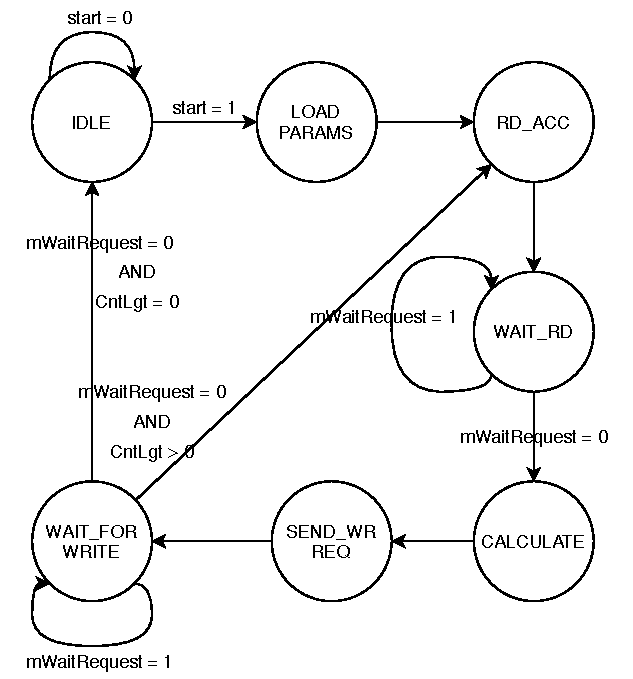
\includegraphics{./pictures/fsm.pdf}}
	\end{center}
	\caption{Finite State Machine states}
	\label{fig:fsm}
\end{figure}

\section{Testing}
VHDL design was tested using ModelSim. Important signals from the test bench code are presented below.
\begin{minted}{vhdl}
nReset <= '0' after period,
          '1' after period + period/2;

sChipSelect <= '1',
               '0' after period*7;
sWrite <= '1',
          '0' after period*7;

-- slave read
sAddress <= "000" after period*2, -- RegAddStart
            "001" after period*3, -- RegLgt
            "011" after period*4, -- ResultRegAddStart
            "010" after period*6; -- start

sWriteData <= x"FFFFFFFF" after period*2, -- RegAddStart
              x"00000004" after period*3, -- RegLgt
              x"AAAAAAAA" after period*4, -- ResultRegAddStart
              x"FFFFFFF1" after period*6; -- start
              -- slave read

-- master 
mReadData <= x"0000000B" after period*10; -- WAIT_RD state

mWaitRequest <= '1' after period*10, -- master looks for the data
                '0' after period*12; -- data in mReadData available 
\end{minted}
\figurename{} \ref{fig:fsm_test_1}, \ref{fig:fsm_test_2}, \ref{fig:fsm_test_3} show wave forms from the subsequent FSM states. 

\begin{sidewaysfigure}
\begin{figure}[H]
	\begin{center}
		\scalebox{0.35}{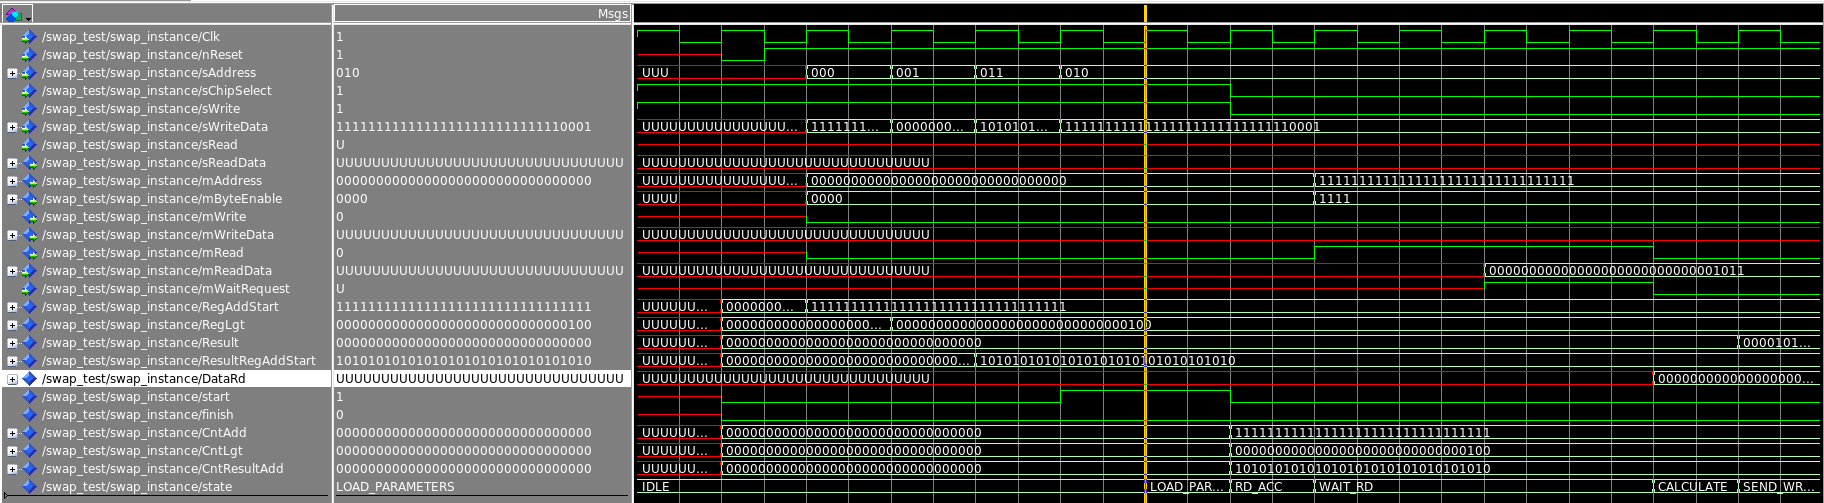
\includegraphics{./pictures/test_1.png}}
	\end{center}
	\caption{Finite State Machine test, states from IDLE to SEND\_WRITE\_REQUEST}

	\label{fig:fsm_test_1}
\end{figure}

\begin{figure}[H]
	\begin{center}
		\scalebox{0.35}{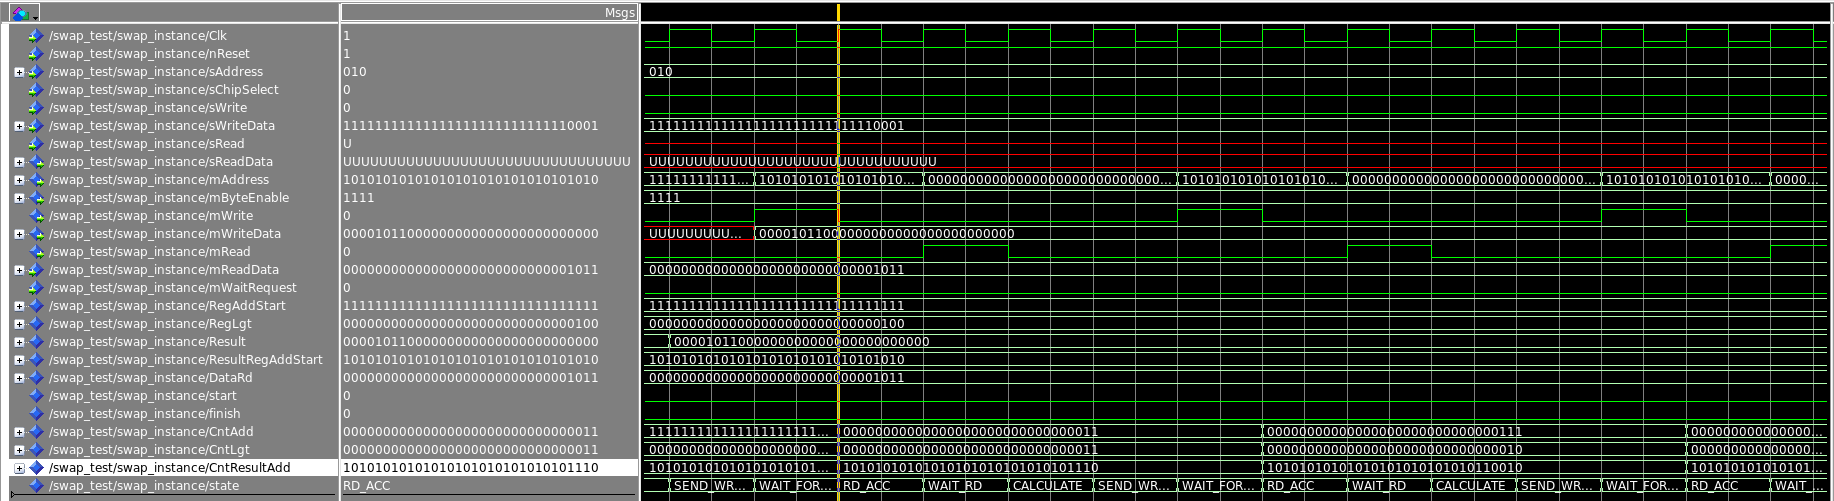
\includegraphics{./pictures/test_2.png}}
	\end{center}
	\caption{Finite State Machine test, states from SEND\_WRITE\_REQUEST to RD\_ACC}

	\label{fig:fsm_test_2}
\end{figure}

\end{sidewaysfigure}

\newpage

\begin{sidewaysfigure}

\begin{figure}[H]
	\begin{center}
		\scalebox{0.35}{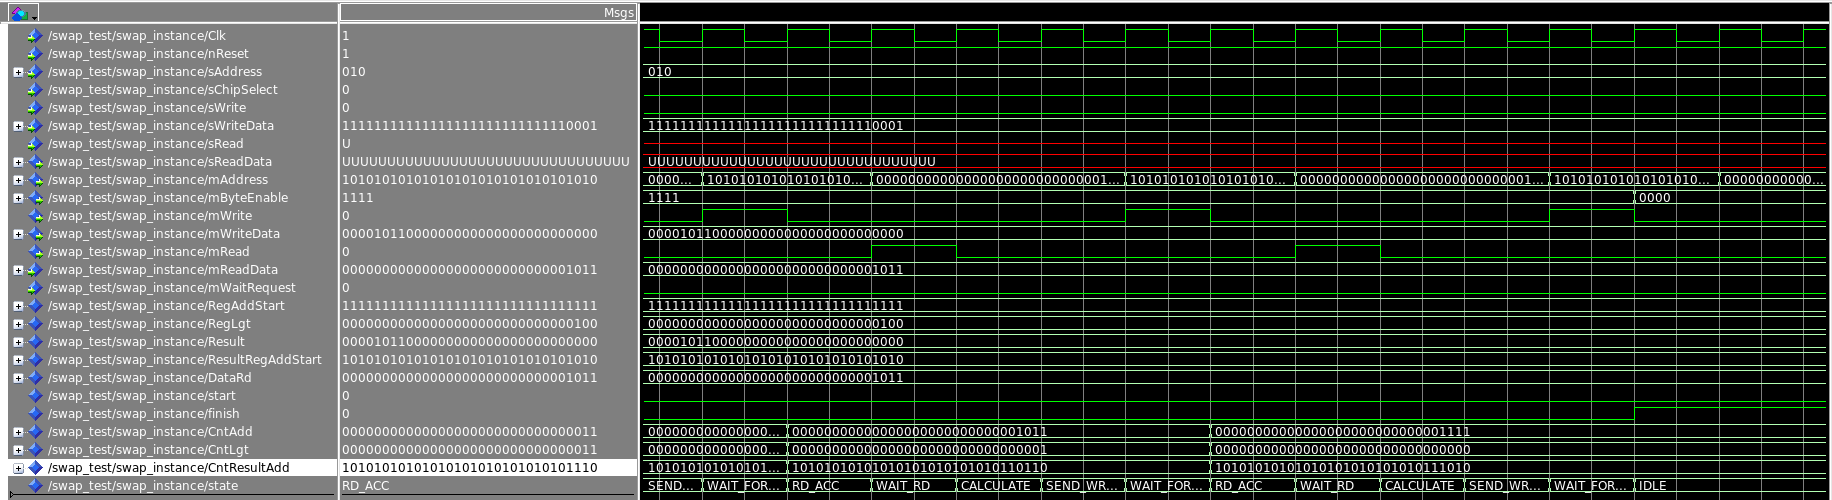
\includegraphics{./pictures/test3.png}}
	\end{center}
	\caption{Finite State Machine test, end of the computation}

	\label{fig:fsm_test_3}
\end{figure}

\end{sidewaysfigure}
\newpage

\figurename{} \ref{fig:fsm_test_1} shows writing into the component with the help of \verb|Avalon| slave signals. Length of the array is set to 4, addresses of the source and result are respectively 1111\dots111, and 1010\dots1010. 
The result of the test bit reshuffling operation can be observed on the \figurename{} \ref{fig:fsm_test_3}.

\section{Software communication with the accelerator}
The following listing shows the function responsible for the communication with the accelerator. It is worth noting that the addresses commands from the top of the listing have to be multiplied by 4 in order to pass them as a first byte in 4 bytes ReadData buffer -- address vector from the design has only 4 bits, hence to put there data properly that data have to be multiplied by 4. 
\begin{lstlisting}[style=customc, frame=none]
#include <stdio.h>
#include <stdbool.h>
#include <stdint.h>
#include <unistd.h>
#include "io.h"
#include "altera_avalon_pio_regs.h"
#include "system.h"
#include "sys/alt_stdio.h"

unsigned int RegAddStart        = 0*4;
unsigned int RegLgt             = 1*4;
unsigned int ResultRegAddStart  = 3*4;
unsigned int start              = 2*4;
unsigned int finish             = 5*4;

void bit_reshuffle_hardware_accelerator(unsigned int *data,
        unsigned int *result, unsigned int size)
{
    // prepare accelerator
    IOWR_32DIRECT(SWAP_ACCELERATOR_0_BASE, RegAddStart, 
        (unsigned int)data);
    IOWR_32DIRECT(SWAP_ACCELERATOR_0_BASE, RegLgt, size);
    IOWR_32DIRECT(SWAP_ACCELERATOR_0_BASE, ResultRegAddStart, 
        (unsigned int)result);
    IOWR_32DIRECT(SWAP_ACCELERATOR_0_BASE, start, 0x00000001); // start
    // wait when the accelerator finishes 
    while(!IORD_32DIRECT(SWAP_ACCELERATOR_0_BASE, finish)) {;}
}
\end{lstlisting}
To ensure that the component can be accessed without problems from the software, a 100 elements array is passed to the accelerator previously initialised with 0x12345678. When the computation is finished result array is printed on the standard output. 

\begin{lstlisting}[style=customc, frame=none]
// main.c
#define size 100 
unsigned int data[size], result[size]; // global

for(int i = 0; i < size; i++) {
    IOWR_32DIRECT(&data[i], 0, 0x12345678);
    IOWR_32DIRECT(&result[i], 0, 0x00000000);
}
bit_reshuffle_hardware_accelerator(&data[0], &result[0], 
    size);
for(int i = 0; i < size; i++){
    printf("result      =0x%x, 0x%x\n", 
        &result[i], IORD_32DIRECT(&result[i], 0));
}
\end{lstlisting}
Result of above code listing is presented below. The element address and the calculation result itself are printed next to one another
\begin{lstlisting}[frame=none]
result      =0x4013894, 0x786a2c12
result      =0x4013898, 0x786a2c12
result      =0x401389c, 0x786a2c12
result      =0x40138a0, 0x786a2c12
result      =0x40138a4, 0x786a2c12
result      =0x40138a8, 0x786a2c12
result      =0x40138ac, 0x786a2c12
\end{lstlisting}

\section{Profiling}
After ensuring, that the hardware accelerator is working properly, its performance was measured by the profiler tool.
\begin{table}[h!]
\centering
\begin{tabular}{    |l|c|c|c|c|c|c|c|  }
\hline
 Amount of bit swaps & 1 & 10 & 100 & 1'000 & 10'000 & 100'000 & 1'000'000\\
 \hline
 Time spent in function [ms]  & $<$ 1  & $<$ 1  & $<$ 1 & $<$ 1 & $<$ 1 & $<$ 1 & 200\\
 \hline
\end{tabular}
 \caption{Timing measurements for hardware accelerator}
\label{table:softwareCodeMeasure}
\end{table}
The hardware accelerator thanks to the direct memory access is much faster than software and has similar performance as custom instruction. 
\begingroup
\renewcommand{\cleardoublepage}{}
\renewcommand{\clearpage}{}
\chapter{Conclusions}
\endgroup
Several important notions were tested within this project. First of all custom instruction and hardware accelerator with direct memory access were implemented in vhdl, tested and exploited for bit reshuffling. Consequently their performance was compared with each other and with pure software implementation of bit reshuffling. Taking into account that the performance of the custom instruction and the hardware accelerator is similar, the conclusion can be that it is better to utilize custom instruction, because it requires much less work and implementation time.However the biggest obstacle surprisingly was the profiler. It was not possible to measure exact performance at some point of the hardware accelerator. The communication is presented on the \figurename{} \ref{gmon}. 

\begin{figure}[H]
	\begin{center}
		\scalebox{0.35}{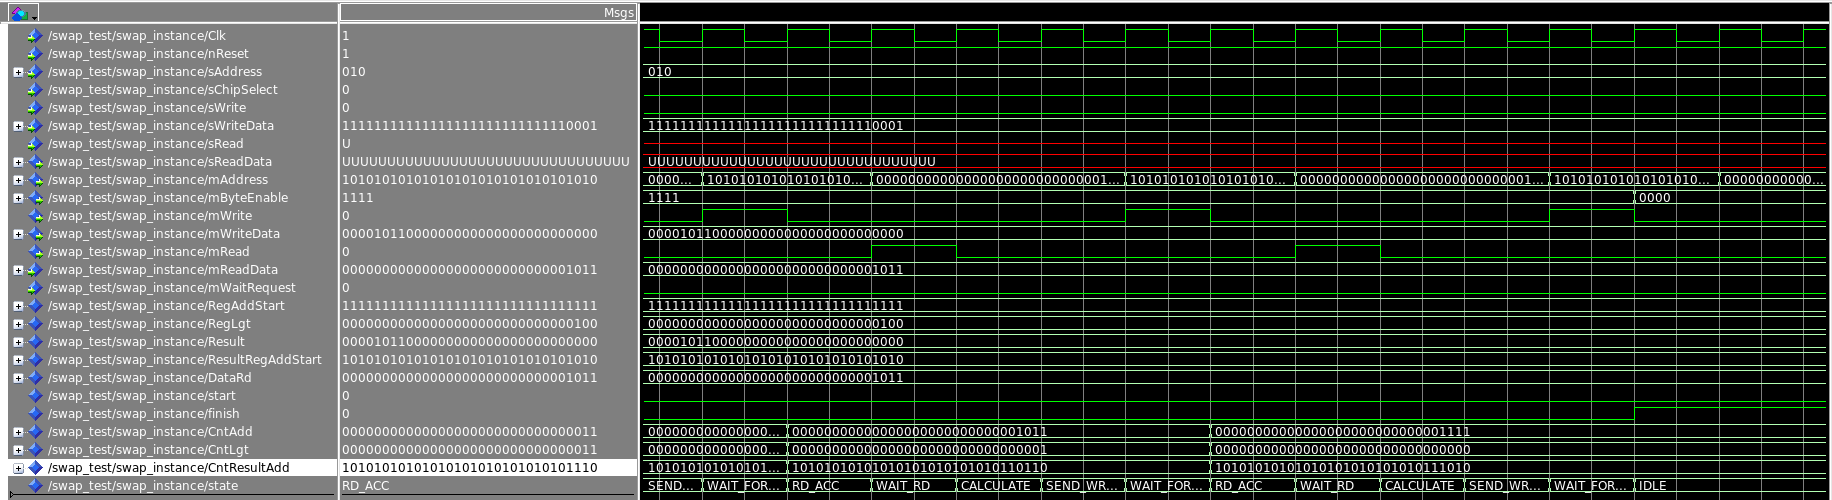
\includegraphics{./pictures/test3.png}}
	\end{center}
	\caption{Finite State Machine test, end of the computation}

	\label{fig:gmon}
\end{figure}